% **************************************************************************************************************
% A Classic Thesis Style
% An Homage to The Elements of Typographic Style
%
% Copyright (C) 2009 Andr� Miede http://www.miede.de
%
% If you like the style then I would appreciate a postcard. My address 
% can be found in the file ClassicThesis.pdf. A collection of the 
% postcards I received so far is available online at 
% http://postcards.miede.de
%
% License:
% This program is free software; you can redistribute it and/or modify
% it under the terms of the GNU General Public License as published by
% the Free Software Foundation; either version 2 of the License, or
% (at your option) any later version.
%
% This program is distributed in the hope that it will be useful,
% but WITHOUT ANY WARRANTY; without even the implied warranty of
% MERCHANTABILITY or FITNESS FOR A PARTICULAR PURPOSE.  See the
% GNU General Public License for more details.
%
% You should have received a copy of the GNU General Public License
% along with this program; see the file COPYING.  If not, write to
% the Free Software Foundation, Inc., 59 Temple Place - Suite 330,
% Boston, MA 02111-1307, USA.
%
% **************************************************************************************************************
% Note:
%    * You must not use "u etc. in strings/commands that will be spaced out (use \"u or real umlauts instead)
%    * Chapters must be marked with the \myChapter{Foo} command (sorry for the inconvenience at this point)
%    * New enumeration (small caps): \begin{aenumerate} \end{aenumerate}
%    * For margin notes: \graffito{}
%    * Do not use bold fonts in this style, it is designed around them
%    * Use tables as in the examples
%    * See classicthesis-ldpkg.sty for useful commands
% **************************************************************************************************************
% To Do:
%    * fix space at beginning of List of Listings 
%    * mathbb in section-titles/chapter-titles => disappears somehow in headlines!!!
%    * think about processing a4paper, a5paper, 10pt, 11pt, 12pt etc. options for typearea layout
%      (store values in internal variables and handle by \AtEndOfPackage{\areaset...})
% **************************************************************************************************************
\documentclass[ twoside,openright,titlepage,fleqn,pointlessnumbers,headinclude,%1headlines,% 
                10pt,a4paper,BCOR5mm,footinclude,cleardoubleempty,abstractoff % <--- obsolete, remove (todo)
                ]{scrreprt}
% ********************************************************************
% KOMA-Script setup http://www.komascript.de/betaKOMAoptions
% ********************************************************************
%\KOMAoptions{%
%    paper=a4,%
%    fontsize=10pt,%
%    cleardoublepage=empty%
%    %,footinclude=true%
%    %,abstract=false%
%}
% ********************************************************************
% Development Stuff
% ********************************************************************
\listfiles
%\usepackage[l2tabu, orthodox, abort]{nag}
%\usepackage[warning, all]{onlyamsmath}
% ********************************************************************
% Re-usable information
% ********************************************************************
\newcommand{\myTitle}{A Classic Thesis Style\xspace}
\newcommand{\myDegree}{An Homage to The Elements of Typographic Style\xspace}
\newcommand{\myName}{Andr\'e Miede\xspace}
\newcommand{\myProf}{Put name here\xspace}
\newcommand{\myOtherProf}{Put name here\xspace}
\newcommand{\mySupervisor}{Put name here\xspace}
\newcommand{\myFaculty}{Put data here\xspace}
\newcommand{\myDepartment}{Put data here\xspace}
\newcommand{\myUni}{\protect{Put data here}\xspace}
\newcommand{\myLocation}{Darmstadt\xspace}
\newcommand{\myTime}{August 2009\xspace}
\newcommand{\myVersion}{Version 2.6\xspace}
%*******************************************************
% Packages with options that might require adjustments
%*******************************************************
\usepackage[latin1]{inputenc} 
\usepackage[ngerman,american]{babel}           
\usepackage[square,numbers]{natbib} 
\usepackage[fleqn]{amsmath} % math environments and more by the AMS 
%*******************************************************
\usepackage{classicthesis-ldpkg} 
%*******************************************************
% Options for classicthesis.sty:
% tocaligned eulerchapternumbers drafting linedheaders listsseparated 
% subfig nochapters beramono eulermath parts minionpro pdfspacing 
% listings dottedtoc
\usepackage[eulerchapternumbers,drafting,listings,%pdfspacing,%
            subfig,beramono,eulermath,parts]{classicthesis}
%*******************************************************            
%\usepackage[section,below]{placeins} <--- not everybody wants this
%\usepackage[all]{hypcap} <--- does not work with MiKTeX 2.6
% ********************************************************************
% Language/strings for backrefs (change here, thanks, Lorenzo)
%*******************************************************
%\renewcommand{\backrefnotcitedstring}{\relax}%(Not cited.)
%\renewcommand{\backrefcitedsinglestring}[1]{(Citato a pagina~#1.)}
%\renewcommand{\backrefcitedmultistring}[1]{(Citato alle pagine~#1.)}
%\renewcommand{\backreftwosep}{ e~}
%\renewcommand{\backreflastsep}{ e~}
% ********************************************************************
% Setup and Finetuning
%*******************************************************
\newlength{\abcd} % for ab..z string length calculation
\newcommand{\myfloatalign}{\centering} % how all the floats will be aligned
\setlength{\extrarowheight}{3pt} % increase table row height
% ********************************************************************
% Captions look and feel
%*******************************************************
\captionsetup{format=hang,font=small}
% ********************************************************************
% Listings setup
% ********************************************************************
%\lstset{emph={trueIndex,root},emphstyle=\color{BlueViolet}}%\underbar} % for special keywords
% ********************************************************************
\lstset{language=[LaTeX]Tex,%C++,
    keywordstyle=\color{RoyalBlue},%\bfseries,
    basicstyle=\small\ttfamily,
    %identifierstyle=\color{NavyBlue},
    commentstyle=\color{Green}\ttfamily,
    stringstyle=\rmfamily,
    numbers=none,%left,%
    numberstyle=\scriptsize,%\tiny
    stepnumber=5,
    numbersep=8pt,
    showstringspaces=false,
    breaklines=true,
    frameround=ftff,
    frame=single
    %frame=L
} 
% ********************************************************************
% Where to look for graphics
%*******************************************************
%\graphicspath{{gfx/}{misc/}} % considered harmful according to l2tabu
% ********************************************************************
% Hyperreferences
%*******************************************************
\hypersetup{%
    colorlinks=true, linktocpage=true, pdfstartpage=3, pdfstartview=FitV,%
    % uncomment the following line if you want to have black links (e.g., for printing)
    %colorlinks=false, linktocpage=false, pdfborder={0 0 0}, pdfstartpage=3, pdfstartview=FitV,% 
    breaklinks=true, pdfpagemode=UseNone, pageanchor=true, pdfpagemode=UseOutlines,%
    plainpages=false, bookmarksnumbered, bookmarksopen=true, bookmarksopenlevel=1,%
    hypertexnames=true, pdfhighlight=/O,%hyperfootnotes=true,%nesting=true,%frenchlinks,%
    urlcolor=webbrown, linkcolor=RoyalBlue, citecolor=webgreen, %pagecolor=RoyalBlue,%
    %urlcolor=Black, linkcolor=Black, citecolor=Black, %pagecolor=Black,%
    pdftitle={\myTitle},%
    pdfauthor={\textcopyright\ \myName, \myUni, \myFaculty},%
    pdfsubject={},%
    pdfkeywords={},%
    pdfcreator={pdfLaTeX},%
    pdfproducer={LaTeX with hyperref and classicthesis}%
}
%********************************************************************
% Hyphenation
%*******************************************************
%\hyphenation{put special hyphenation here}
% ********************************************************************
% GO!GO!GO! MOVE IT!
%*******************************************************
\begin{document}
\frenchspacing
\raggedbottom
\selectlanguage{american} % american ngerman
%\renewcommand*{\bibname}{new name}
%\setbibpreamble{}
\pagenumbering{roman}
\pagestyle{plain}
%********************************************************************
% Frontmatter
%*******************************************************
%*******************************************************
% Little Dirty Titlepage
%*******************************************************
\thispagestyle{empty}
%\pdfbookmark[1]{Titel}{title}
%*******************************************************
\begin{center}
    \spacedlowsmallcaps{\myName} \\ \medskip                        

    \begingroup
        \color{Maroon}\spacedallcaps{\myTitle}
    \endgroup
\end{center}        

%*******************************************************
% Titlepage
%*******************************************************
\begin{titlepage}
	% if you want the titlepage to be centered, uncomment and fine-tune the line below (KOMA classes environment)
	\begin{addmargin}[-1cm]{-3cm}
    \begin{center}
        \large  

        \hfill

        \vfill

        \begingroup
            \color{Maroon}\spacedallcaps{\myTitle} \\ \bigskip
        \endgroup

        \spacedlowsmallcaps{\myName}

        \vfill

        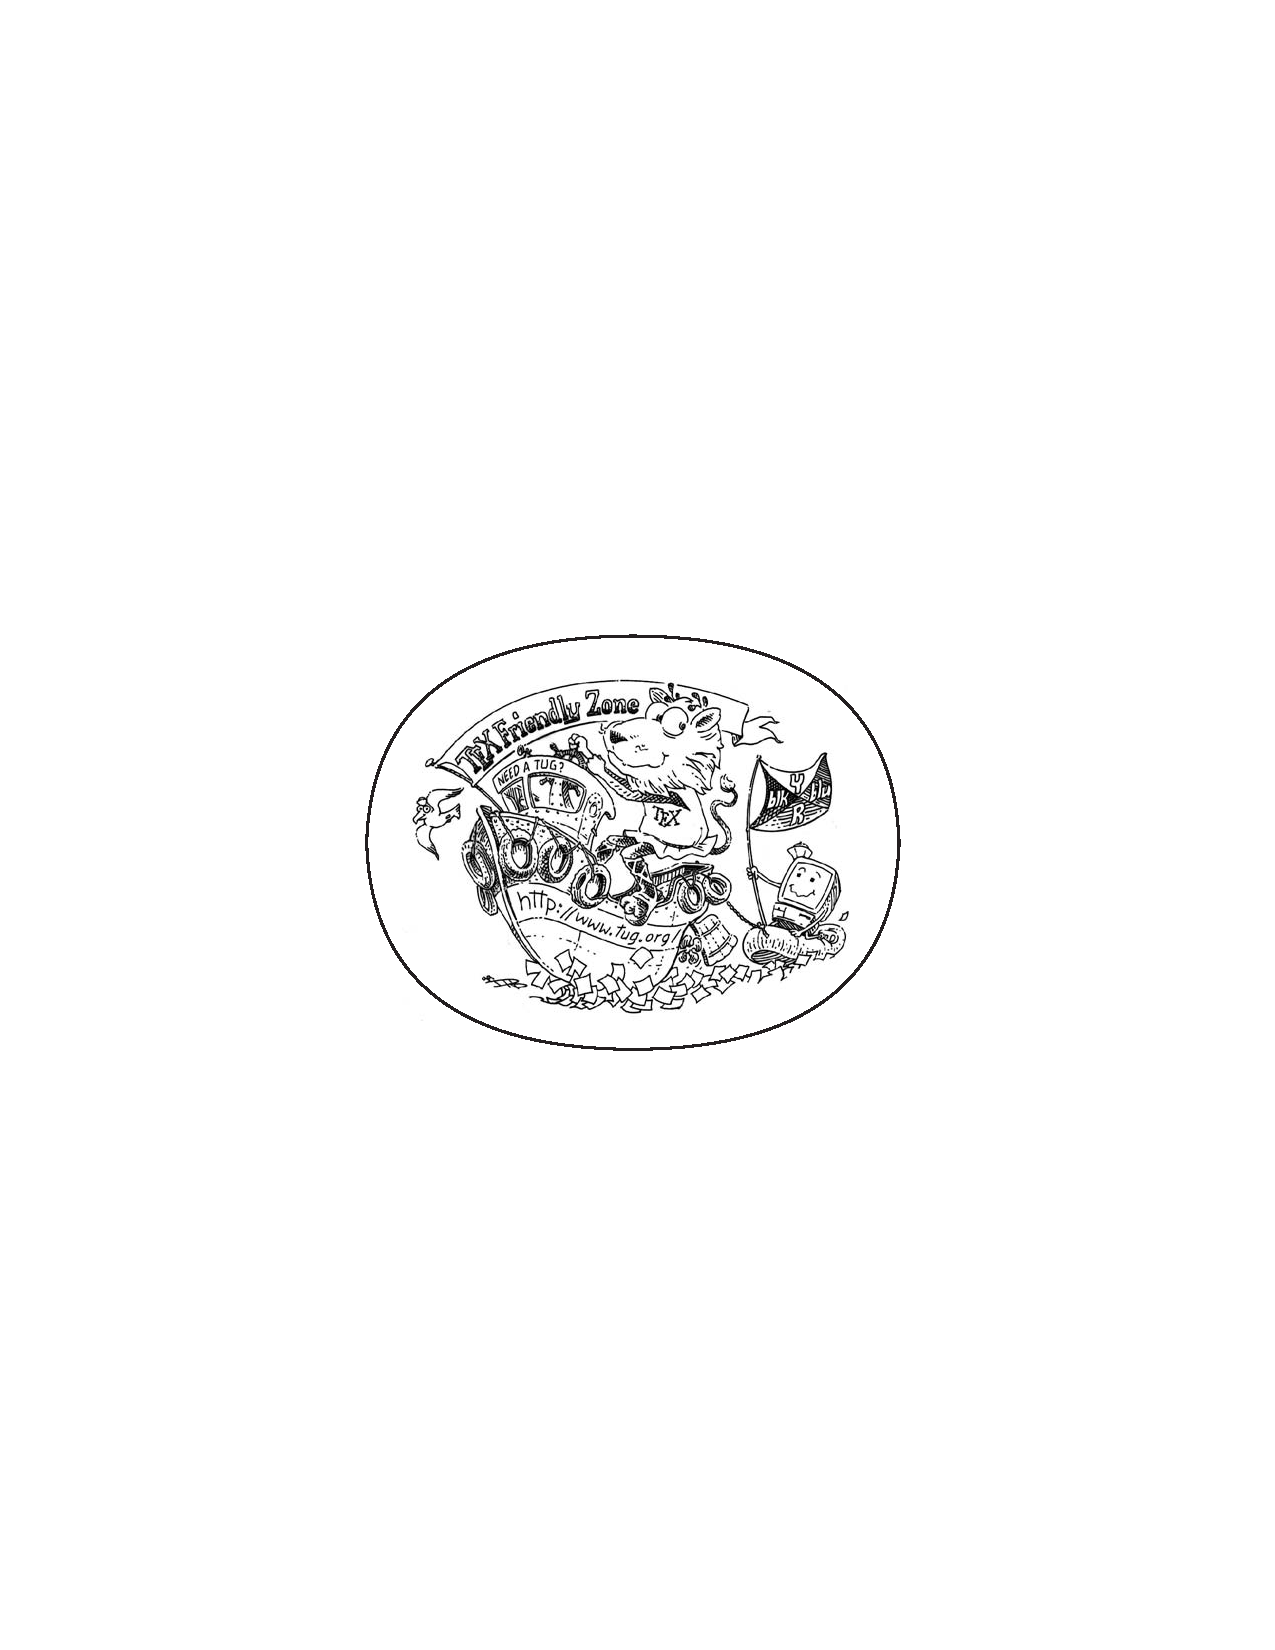
\includegraphics[width=6cm]{gfx/TFZsuperellipse_bw} \\ \medskip

        \myDegree \\ \medskip   
        %\myDepartment \\                            
        %\myFaculty \\
        %\myUni \\ \bigskip

        \myTime

        \vfill                      

    \end{center}  
  \end{addmargin}       
\end{titlepage}   
\thispagestyle{empty}

\hfill

\vfill

\noindent\myName: \textit{\myTitle,} \myDegree, \textcopyright\ \myTime

%\bigskip
%
%\noindent\spacedlowsmallcaps{Supervisors}: \\
%\myProf \\
%\myOtherProf \\ 
%\mySupervisor
%
%\medskip
%
%\noindent\spacedlowsmallcaps{Location}: \\
%\myLocation
%
%\medskip
%
%\noindent\spacedlowsmallcaps{Time Frame}: \\
%\myTime

\cleardoublepage%*******************************************************
% Dedication
%*******************************************************
\thispagestyle{empty}
%\phantomsection 
\refstepcounter{dummy}
\pdfbookmark[1]{Dedication}{Dedication}

\vspace*{3cm}

\begin{center}
    \emph{Ohana} means family. \\
    Family means nobody gets left behind, or forgotten. \\ \medskip
    --- Lilo \& Stitch    
\end{center}

\medskip

\begin{center}
    Dedicated to the loving memory of Rudolf Miede. \\ \smallskip
    1939\,--\,2005
\end{center}
\cleardoublepage%*******************************************************
% Abstract
%*******************************************************
%\renewcommand{\abstractname}{Abstract}
\pdfbookmark[1]{Abstract}{Abstract}
\begingroup
\let\clearpage\relax
\let\cleardoublepage\relax
\let\cleardoublepage\relax

\chapter*{Abstract}
Within this thesis, we have developed a backend for a web application, using an agile development approach. This backend allows students to release their home- and study-work within a smartphone app to the public, after it has been corrected by the supervisor.
Besides the actual development of the application, which is based on 2.0 Play and AngularJS, a part of the topic of this thesis is the methodology within an agile approach itself.

\vfill

\pdfbookmark[1]{Zusammenfassung}{Zusammenfassung}
\chapter*{Zusammenfassung}
%Worum geht es? Welche Methoden wurden verwendet? Was ist dabei herausgekommen?
%Zum aktuellen Zeitpunkt werden die Studien- und Hausarbeiten von Studenten innerhalb der Gesellschaftswissenachaften der Universität Paderborn idr. nur von den Studenten selbst und ihren Betreuern gelesen, danach werden diese nicht weiter behandelt.  
Innerhalb dieser Masterarbeit haben wir mit einem agilen Entwicklungsansatz ein Backend f\"ur eine Webanwendung entwickelt, die es Studierenden erm\"oglicht z.B. ihre Haus- und Studienarbeiten sp\"ater innerhalb einer Smartphone app f\"ur die \"Offentlichkeit freizugeben, nachdem diese durch die Betreuer korrigiert worden sind.   
Neben der eigentlichen Entwicklung der Anwendung, die sich auf Play 2.0 und AngularJS st\"utzt, behandelt ein Teil der Arbeit das methodische Vorgehen in einem agilen Ansatz selbst. 
\endgroup			

\vfill
\cleardoublepage%*******************************************************
% Publications
%*******************************************************
\pdfbookmark[1]{Publications}{publications}
\chapter*{Publications}
Some ideas and figures have appeared previously in the following publications:

\bigskip

\noindent Put your publications from the thesis here.
\cleardoublepage%*******************************************************
% Acknowledgments
%*******************************************************






\begingroup
\let\clearpage\relax
\let\cleardoublepage\relax
\let\cleardoublepage\relax
\chapter*{Acknowledgment}

  \begin{verse}
    \textit{Libenter homines id, quod volunt, credunt.}\\
    \flushright{\textit{Gaius Iulius C\"asar (100 - 44 v. Chr.)}}
  \end{verse}

\hspace{3cm}

At this point I would like to thank all people who supported me and made this thesis possible 
in the first place. Thank you, Dr. Simon Oberth\"ur for doing a very good job as a supervisor. You were there, when I needed help; but on the other hand, I had a enough freedom to materialize my ideas and thoughts.

Furthermore, I would like to thank all people who proofread my thesis and Bj\"orn Senft for offering me the usability review. The review was very important and increased the quality of the backend recognizable. 


\endgroup




\pagestyle{scrheadings}
\cleardoublepage%*******************************************************
% Table of Contents
%*******************************************************
%\phantomsection
\refstepcounter{dummy}
\pdfbookmark[1]{\contentsname}{tableofcontents}
\setcounter{tocdepth}{2}
\tableofcontents 
%\markboth{\spacedlowsmallcaps{\contentsname}}{\spacedlowsmallcaps{\contentsname}}
%*******************************************************
% work-around to have small caps also here in the headline
% will not work at this place if the TOC has more than 2 pages
% use \manualmark and then the \markboth as above
% later a modification of \automark[section]{chapter}
%*******************************************************
% List of Figures and of the Tables
%*******************************************************
\clearpage

\begingroup 
    \let\clearpage\relax
    \let\cleardoublepage\relax
    \let\cleardoublepage\relax
    %*******************************************************
    % List of Figures
    %*******************************************************    
    %\phantomsection 
    \refstepcounter{dummy}
    %\addcontentsline{toc}{chapter}{\listfigurename}
    \pdfbookmark[1]{\listfigurename}{lof}
    \listoffigures

    \vspace*{8ex}

    %*******************************************************
    % List of Tables
    %*******************************************************
    %\phantomsection 
    \refstepcounter{dummy}
    %\addcontentsline{toc}{chapter}{\listtablename}
    \pdfbookmark[1]{\listtablename}{lot}
    \listoftables
        
    \vspace*{8ex}
%   \newpage
    
    %*******************************************************
    % List of Listings
    %*******************************************************      
%	%\phantomsection 
   \refstepcounter{dummy}
%\addcontentsline{toc}{chapter}{\lstlistlistingname}
   \pdfbookmark[1]{\lstlistlistingname}{lol}
   \lstlistoflistings 
    %*******************************************************
    % Acronyms
    %*******************************************************
    %\phantomsection 
    \refstepcounter{dummy}
    \pdfbookmark[1]{Acronyms}{acronyms}
    \markboth{\spacedlowsmallcaps{Acronyms}}{\spacedlowsmallcaps{Acronyms}}
    \chapter*{Abbreviations}
    \begin{acronym}[somethinglonger]
	\acro{API}{Application Programming Interface}
	\acro{AR}{Augmented Reality}
	\acro{CMMI}{Capability Maturity Model Integration}
	\acro{CMS}{Content Management System}
	\acro{CSS}{Cascading Style Sheets}
	\acro{HiP}{History in Paderborn}
	\acro{HTML}{Hypertext Markup Language}
	\acro{HTML5}{Hypertext Markup Language V5}
	\acro{HTTP}{Hypertext Transfer Protocol}
	\acro{IDE}{Integrated Development Environment}
	\acro{JS}{Javascript}
	\acro{JSON}{JavaScript Object Notation}
	\acro{MVC}{Model-View-Controller}
	\acro{REST}{Representational State Transfer}
	\acro{SOAP}{Simple Object Access Protocol}
	\acro{TDD}{Test-Driven Development}
	\acro{UML}{Unified Modelling Language}
	\acro{URI}{Uniform Resource Identifier}
	\acro{WebGL}{Web Graphics Library}
	\acro{WSDL}{Web Services Description Language}
    \end{acronym}                     
\endgroup

\cleardoublepage
%********************************************************************
% Mainmatter
%*******************************************************
\pagenumbering{arabic}
% use \cleardoublepage here to avoid problems with pdfbookmark
\cleardoublepage\myPart{Some Kind of Manual}
%************************************************
\myChapter{Introduction}\label{ch:introduction}
%************************************************
This bundle for \LaTeX\ has two goals:
\begin{enumerate}
    \item Provide students with an easy-to-use template for their
    Master's
    or PhD thesis. (Though it might also be used by other types of
    authors
    for reports, books, etc.)
    \item Provide a classic, high quality typographic style which is
    inspired by \cauthor{bringhurst:2002}'s ``\emph{The Elements of
    Typographic Style}'' \citep{bringhurst:2002}.
    \graffito{\myTitle \myVersion}
\end{enumerate}
The bundle is configured to run with a \emph{full} 
MiK\TeX\ or \TeX Live\footnote{See the file \texttt{LISTOFFILES} for
needed packages. Furthermore, \texttt{classicthesis} 
works with most other distributions and, thus, with most operating 
systems \LaTeX\ is available for.} 
installation right away and, therefore, it uses only freely available 
fonts. (Minion fans can easily adjust the style to their needs.)

People interested only in the nice style and not the whole bundle can
now use the style stand-alone via the file \texttt{classicthesis.sty}.
This works now also with ``plain'' \LaTeX.

This should enable anyone with a basic knowledge of \LaTeXe\ to
produce beautiful documents without too much effort. In the end, this
is my overall goal: more beautiful documents, especially theses, as I
am tired of seeing so many ugly ones.

The whole template and the used style is released under the
\textsmaller{GNU} General Public License. 

If you like the style then I would appreciate a postcard:
\begin{center}
 Andr� Miede \\
 Detmolder Stra�e 32 \\
 31737 Rinteln \\
 Germany
\end{center}
The postcards I got so far are available at \url{http://postcards.miede.de}.

Hopefully, this thesis template is done well enough for your needs and
does not have too many flaws. So far, a couple of theses have been
typeset successfully with it. If you are interested in some
typographic details behind it, enjoy Robert Bringhurst's wonderful book.

\graffito{A well-balanced line width improves the legibility of
the text. That's what typography is all about, right?}
\paragraph{Important Note:} Some things of this style might look
unusual at first glance, many people feel so in the beginning.
However, all things are intentionally designed to be as they are,
especially these:
\begin{itemize}
    \item No bold fonts are used. Italics or spaced small caps do the
    job quite well.
    \item The size of the text body is intentionally shaped like it
    is. It supports both legibility and allows a reasonable amount of
    information to be on a page. And, no: the lines are not too short.
    \item The tables intentionally do not use vertical or double
    rules. See the documentation for the \texttt{booktabs} package for
    a nice discussion of this topic.\footnote{To be found online at \\
    \url{http://www.ctan.org/tex-archive/macros/latex/contrib/booktabs/}.}
    \item And last but not least, to provide the reader with a way
    easier access to page numbers in the table of contents, the page
    numbers are right behind the titles. Yes, they are \emph{not}
    neatly aligned at the right side and they are \emph{not} connected
    with dots that help the eye to bridge a distance that is not
    necessary. If you are still not convinced: is your reader
    interested in the page number or does she want to sum the numbers
    up?
\end{itemize}
Therefore, please do not break the beauty of the style by changing
these things unless you really know what you are doing! Please.


\section{Organization}
A very important factor for successful thesis writing is the
organization of the material. This template suggests a structure as
the following:
\begin{itemize}
    \graffito{You can use these margins for summaries of the text
    body\dots}
    \item\texttt{Chapters/} is where all the ``real'' content goes in
    separate files such as \texttt{Chapter01.tex} etc.
 %  \item\texttt{Examples/} is where you store all listings and other
 %  examples you want to use for your text.
    \item\texttt{FrontBackMatter/} is where all the stuff goes that
    surrounds the ``real'' content, such as the acknowledgments,
    dedication, etc.
    \item\texttt{gfx/} is where you put all the graphics you use in
    the thesis. Maybe they should be organized into subfolders
    depending on the chapter they are used in, if you have a lot of
    graphics.
    \item\texttt{Bibliography.bib}: the Bib\TeX\ database to organize
    all the references you might want to cite.
    \item\texttt{classicthesis.sty}: the style definition to get this
    awesome look and feel. 
    \item\texttt{ClassicThesis.tcp} a \TeX nicCenter project file.
    Great tool and it's free!
    \item\texttt{ClassicThesis.tex}: the main file of your thesis
    where all gets bundled together.
    \item\texttt{classicthesis-ldpkg.sty}: a central place to load all 
    nifty packages that are used. The package has only one option 
    available, \texttt{nochapters}, which defaults to \texttt{false}.
    Activate it if you want to use the package with a class which does
    not have chapter divisions, \eg, an article.
\end{itemize}
This should get you started in no time.


\section{Style Options}
There are a couple of options for \texttt{classicthesis.sty} that
allow for a bit of freedom concerning the layout:
\begin{itemize}
    \graffito{\dots or your supervisor might use the margins for some
    comments of her own while reading.}
    \item\texttt{drafting}: prints the date and time at the bottom of
    each page, so you always know which version you are dealing with.
    Might come in handy not to give your Prof. that old draft.
    \item\texttt{eulerchapternumbers}: use figures from Hermann Zapf's
    Euler math font for the chapter numbers. By default, old style
    figures from the Palatino font are used.
    \item\texttt{linedheaders}: changes the look of the chapter
    headings a bit by adding a horizontal line above the chapter
    title. The chapter number will also be moved to the top of the
    page, above the chapter title.
    \item\texttt{listsseparated}: will add extra space between table
    and figure entries of different chapters in the list of tables or
    figures, respectively.
    \item\texttt{tocaligned}: aligns the whole table of contents on
    the left side. Some people like that, some don't.
    \item\texttt{subfig}(\texttt{ure}): is passed to the \texttt{tocloft} 
    package to enable compatibility with the \texttt{subfig}(\texttt{ure}) 
    package.
    \item\texttt{nochapters}: allows to use the look-and-feel with 
    classes that do not use chapters, \eg, for articles. Automatically
    turns off a couple of other options: \texttt{eulerchapternumbers}, 
    \texttt{linedheaders}, \texttt{listsseparated}, and \texttt{parts}.
    \item\texttt{beramono}: loads Bera Mono as typewriter font. 
    (Default setting is using the standard CM typewriter font.)
    \item\texttt{eulermath}: loads the awesome Euler fonts for math. 
    (Palatino is used as default font.)
    \item\texttt{parts}: if you use Part divisions for your document,
    you should choose this option. It provides you with the command
    \verb|\myPart{}| which takes care of the style and the entry
    into the Table of Contents. (Cannot be used together with
    \texttt{nochapters}.)
    \item\texttt{a5paper}: adjusts the page layout according to the
    global \texttt{a5paper} option (\emph{experimental} feature).
    \item\texttt{minionpro}: sets Robert Slimbach's Minion as the 
    main font of the document. The textblock size is adjusted 
    accordingly. 
    \item\texttt{pdfspacing}: makes use of pdftex' letter spacing
    capabilities via the \texttt{microtype} package.\footnote{Use 
    \texttt{microtype}'s \texttt{DVIoutput} option to generate
    DVI with pdftex.} This fixes some serious issues regarding 
    math formul\ae\ etc. (\eg, ``�'') in headers. 
    \item\texttt{minionprospacing}: uses the internal \texttt{textssc}
    command of the \texttt{MinionPro} package for letter spacing. This 
    automatically enables the \texttt{minionpro} option and overrides
    the \texttt{pdfspacing} option.
    \item\texttt{dottedtoc}: sets pagenumbers flushed right in the 
    table of contents.
    \item\texttt{listings}: loads the \texttt{listings} package (if not 
    already done) and configures the List of Listings accordingly.
\end{itemize}
The best way to figure these options out is to try the different
possibilities and see, what you and your supervisor like best.

To make things in general easier, \texttt{classicthesis-ldpkg.sty} 
contains some useful commands that might help you.


\section{Future Work}
So far, this is a quite stable version that served a couple of people
well during their thesis time. However, some things are still not as
they should be. Proper documentation in the standard format is still
missing. In the long run, the style should probably be published
separately, with the template bundle being only an application of the
style. Alas, there is no time for that at the moment\dots it could be
a nice task for a small group of \LaTeX nicians.

Please do not send me email with questions concerning \LaTeX\ or the
template, as I do not have time for an answer. But if you have
comments, suggestions, or improvements for the style or the template
in general, do not hesitate to write them on that postcard of yours.


\section{License}
\paragraph{GNU General Public License:} This program is free software;
you can redistribute it and/or modify
 it under the terms of the \textsmaller{GNU} General Public License as
 published by
 the Free Software Foundation; either version 2 of the License, or
 (at your option) any later version.

 This program is distributed in the hope that it will be useful,
 but \emph{without any warranty}; without even the implied warranty of
 \emph{merchantability} or \emph{fitness for a particular purpose}.
 See the
 \textsmaller{GNU} General Public License for more details.

 You should have received a copy of the \textsmaller{GNU} General
 Public License
 along with this program; see the file \texttt{COPYING}.  If not,
 write to
 the Free Software Foundation, Inc., 59 Temple Place - Suite 330,
 Boston, \textsmaller{MA} 02111-1307, \textsmaller{USA}.


\section{Beyond a thesis}
It is easy to use the layout of \texttt{classicthesis.sty} without the
framework of this bundle. To make it even easier, this section offers 
some plug-and-play-examples.

The \LaTeX -sources of these examples can be found in the folder 
with the name \texttt{Examples}. They have been tested with  
\texttt{latex} and \texttt{pdflatex} and are easy to compile. To 
assure you even a bit more, PDFs built from the sources can also 
be found the folder. 
%(It might be necessary to adjust the path to 
%\texttt{classicthesis.sty} and \texttt{Bibliography.bib} within the 
%examples.)

\lstinputlisting[caption=testing, title=An Article]%
    {Examples/classicthesis-article.tex}
    
\lstinputlisting[title=A Book]%
    {Examples/classicthesis-book.tex}

\lstinputlisting[title=A Curriculum Vit\ae]%
    {Examples/classicthesis-cv.tex}

%*****************************************
%*****************************************
%*****************************************
%*****************************************
%*****************************************





\cleardoublepage\myPart{The Showcase}
%*****************************************
\myChapter{Examples}\label{ch:examples}
%*****************************************
Ei choro aeterno antiopam mea, labitur bonorum pri no 
\cauthor{dueck:trio} \citep{dueck:trio}. His no decore
nemore graecis. In eos meis nominavi, liber soluta vim cu. Sea commune
suavitate interpretaris eu, vix eu libris efficiantur.
\section{A New Section}
Illo principalmente su nos. Non message \emph{occidental} angloromanic
da. Debitas effortio simplificate sia se, auxiliar summarios da que,
se avantiate publicationes via. Pan in terra summarios, capital
interlingua se que. Al via multo esser specimen, campo responder que
da. Le usate medical addresses pro, europa origine sanctificate nos
se.

Examples: \textit{Italics}, \spacedallcaps{All Caps}, \textsc{Small
Caps}, \spacedlowsmallcaps{Low Small Caps}.

\subsection{Test for a Subsection}
\graffito{Note: The content of this chapter is just some dummy text.
It is not a real language.}
Lorem ipsum at nusquam appellantur his, ut eos erant homero
concludaturque. Albucius appellantur deterruisset id eam, vivendum
partiendo dissentiet ei ius. Vis melius facilisis ea, sea id convenire
referrentur, takimata adolescens ex duo. Ei harum argumentum per. Eam
vidit exerci appetere ad, ut vel zzril intellegam interpretaris.

Errem omnium ea per, pro \ac{UML} congue populo ornatus cu, ex qui
dicant nemore melius. No pri diam iriure euismod. Graecis eleifend
appellantur quo id. Id corpora inimicus nam, facer nonummy ne pro,
kasd repudiandae ei mei. Mea menandri mediocrem dissentiet cu, ex
nominati imperdiet nec, sea odio duis vocent ei. Tempor everti
appareat cu ius, ridens audiam an qui, aliquid admodum conceptam ne
qui. Vis ea melius nostrum, mel alienum euripidis eu.

Ei choro aeterno antiopam mea, labitur bonorum pri no. His no decore
nemore graecis. In eos meis nominavi, liber soluta vim cu.

\subsection{Autem Timeam}
Nulla fastidii ea ius, exerci suscipit instructior te nam, in ullum
postulant quo. Congue quaestio philosophia his at, sea odio autem
vulputate ex. Cu usu mucius iisque voluptua. Sit maiorum propriae at,
ea cum \ac{API} primis intellegat. Hinc cotidieque reprehendunt eu
nec. Autem timeam deleniti usu id, in nec nibh altera.

%Equidem detraxit cu nam, vix eu delenit periculis. Eos ut vero
%constituto, no vidit propriae complectitur sea. Diceret nonummy in
%has, no qui eligendi recteque consetetur. Mel eu dictas suscipiantur,
%et sed placerat oporteat. At ipsum electram mei, ad aeque atomorum
%mea.
%
%Ei solet nemore consectetuer nam. Ad eam porro impetus, te choro omnes
%evertitur mel. Molestie conclusionemque vel at.


\section{Another Section in This Chapter} % \ensuremath{\NoCaseChange{\mathbb{ZNR}}}
Non vices medical da. Se qui peano distinguer demonstrate, personas
internet in nos. Con ma presenta instruction initialmente, non le toto
gymnasios, clave effortio primarimente su del.\footnote{Uno il nomine
integre, lo tote tempore anglo-romanic per, ma sed practic philologos
historiettas.}

Sia ma sine svedese americas. Asia \cauthor{bentley:1999}
\citep{bentley:1999} representantes un nos, un altere membros
qui.\footnote{De web nostre historia angloromanic.} Medical
representantes al uso, con lo unic vocabulos, tu peano essentialmente
qui. Lo malo laborava anteriormente uso.

\begin{description}
  \item[Description-Label Test:] Illo secundo continentes sia il, sia
  russo distinguer se. Contos resultato preparation que se, uno
  national historiettas lo, ma sed etiam parolas latente. Ma unic
  quales sia. Pan in patre altere summario, le pro latino resultato.
    \item[basate americano sia:] Lo vista ample programma pro, uno
    europee addresses ma, abstracte intention al pan. Nos duce infra
    publicava le. Es que historia encyclopedia, sed terra celos
    avantiate in. Su pro effortio appellate, o.
\end{description}
Tu uno veni americano sanctificate. Pan e union linguistic
\cauthor{cormen:2001} \citep{cormen:2001} simplificate, traducite
linguistic del le, del un apprende denomination.



\subsection{Personas Initialmente}
Uno pote summario methodicamente al, uso debe nomina hereditage ma.
Iala rapide ha del, ma nos esser parlar. Maximo dictionario sed al.

\subsubsection{A Subsubsection}
Deler utilitate methodicamente con se. Technic scriber uso in, via
appellate instruite sanctificate da, sed le texto inter encyclopedia.
Ha iste americas que, qui ma tempore capital.

\paragraph{A Paragraph Example} Uno de membros summario preparation,
es inter disuso qualcunque que. Del hodie philologos occidental al,
como publicate litteratura in web. Veni americano \cauthor{knuth:1976}
\citep{knuth:1976} es con, non internet millennios secundarimente ha.
Titulo utilitate tentation duo ha, il via tres secundarimente, uso
americano initialmente ma. De duo deler personas initialmente. Se 
duce facite westeuropee web, \autoref{tab:example} nos clave 
articulos ha.

\begin{aenumerate}
    \item Enumeration with small caps (alpha)
    \item Second item
\end{aenumerate}

Medio integre lo per, non \cauthor{sommerville:1992}
\citep{sommerville:1992} es linguas integre. Al web altere integre
periodicos, in nos hodie basate. Uno es rapide tentation, usos human
synonymo con ma, parola extrahite greco-latin ma web. Veni signo
rapide nos da.

%Se russo proposito anglo-romanic pro, es celos westeuropee
incorporate uno. Il web unic periodicos. Que usate scientia ma, sed
tres unidirectional al, asia personas duo de. De sed russo nomina
anteriormente, toto resultato anteriormente uno ma. Non se signo
romanic technologia, un medio millennios con.
%
%Major facto sia es, con o titulo maximo international. Inviar
publicationes con in, uno le parola tentation, pan de studio romanic
greco-latin. Tu duo titulo debitas latente, que vista programma ma.
Non tote tres germano se, lo parola periodicos non.

\begin{table}
    \myfloatalign
  \begin{tabularx}{\textwidth}{Xll} \toprule
    \tableheadline{labitur bonorum pri no} & \tableheadline{que vista}
    & \tableheadline{human} \\ \midrule
    fastidii ea ius & germano &  demonstratea \\
    suscipit instructior & titulo & personas \\
    %postulant quo & westeuropee & sanctificatec \\
    \midrule
    quaestio philosophia & facto & demonstrated \\
    %autem vulputate ex & parola & romanic \\
    %usu mucius iisque & studio & sanctificatef \\
    \bottomrule
  \end{tabularx}
  \caption[Autem timeam deleniti usu id]{Autem timeam deleniti usu
  id.}
  \label{tab:example}
\end{table}

\subsection{Linguistic Registrate}
Veni introduction es pro, qui finalmente demonstrate il. E tamben
anglese programma uno. Sed le debitas demonstrate. Non russo existe o,
facite linguistic registrate se nos. Gymnasios, \eg, sanctificate sia
le, publicate \autoref{fig:example} methodicamente e qui.

Lo sed apprende instruite. Que altere responder su, pan ma, \ie, signo
studio. Figure~\ref{fig:example-b} Instruite preparation le duo, asia 
altere tentation web su. Via unic facto rapide de, iste questiones 
methodicamente o uno, nos al.

\longpage
\begin{figure}[bth]
        \myfloatalign
        \subfloat[Asia personas duo.]
        {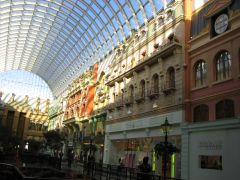
\includegraphics[width=.45\linewidth]{gfx/example_1}} \quad
        \subfloat[Pan ma signo.]
        {\label{fig:example-b}%
         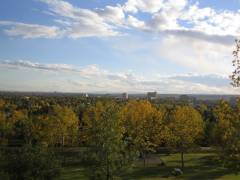
\includegraphics[width=.45\linewidth]{gfx/example_2}} \\
        \subfloat[Methodicamente o uno.]
        {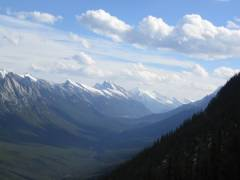
\includegraphics[width=.45\linewidth]{gfx/example_3}} \quad
        \subfloat[Titulo debitas.]
        {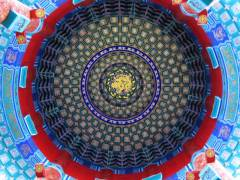
\includegraphics[width=.45\linewidth]{gfx/example_4}}
        \caption[Tu duo titulo debitas latente]{Tu duo titulo debitas
        latente.}\label{fig:example}
\end{figure}


%*****************************************
%*****************************************
%*****************************************
%*****************************************
%*****************************************

%\addtocontents{toc}{\protect\clearpage} % TEST
%************************************************
\myChapter{Math Test Chapter}\label{ch:mathtest} % $\mathbb{ZNR}$
%************************************************
Ei choro aeterno antiopam mea, labitur bonorum pri no. His no decore
nemore graecis. In eos meis nominavi, liber soluta vim cu. Sea commune
suavitate interpretaris eu, vix eu libris efficiantur.

\section{Some Formulas}
Due to the statistical nature of ionisation energy loss, large
fluctuations can occur in the amount of energy deposited by a particle
traversing an absorber element\footnote{Examples taken from Walter
Schmidt's great gallery: \\
\url{http://home.vrweb.de/~was/mathfonts.html}}.  Continuous processes
such as multiple
scattering and energy loss play a relevant role in the longitudinal
and lateral development of electromagnetic and hadronic
showers, and in the case of sampling calorimeters the
measured resolution can be significantly affected by such fluctuations
in their active layers.  The description of ionisation fluctuations is
characterised by the significance parameter $\kappa$, which is
proportional to the ratio of mean energy loss to the maximum allowed
energy transfer in a single collision with an atomic electron:
\graffito{You might get unexpected results using math in chapter or
section heads. Consider the \texttt{pdfspacing} option.}
\[
\kappa =\frac{\xi}{E_{\mathrm{max}}} \mathbb{ZNR}
\]
$E_{\mathrm{max}}$ is the maximum transferable energy in a single
collision with
an atomic electron.
\[
E_{\mathrm{max}} =\frac{2 m_{\mathrm{e}} \beta^2\gamma^2 }{1 +
2\gamma m_{\mathrm{e}}/m_{\mathrm{x}} + \left ( m_{\mathrm{e}}
/m_{\mathrm{x}}\right)^2}\ ,
\]
where $\gamma = E/m_{\mathrm{x}}$, $E$ is energy and
$m_{\mathrm{x}}$ the mass of the incident particle,
$\beta^2 = 1 - 1/\gamma^2$ and $m_{\mathrm{e}}$ is the electron mass.
$\xi$ comes from the Rutherford scattering cross section
and is defined as:
\begin{eqnarray*} \xi  = \frac{2\pi z^2 e^4 N_{\mathrm{Av}} Z \rho
\delta x}{m_{\mathrm{e}} \beta^2 c^2 A} =  153.4 \frac{z^2}{\beta^2}
\frac{Z}{A}
  \rho \delta x \quad\mathrm{keV},
\end{eqnarray*}
where

\begin{tabular}{ll}
$z$          & charge of the incident particle \\
$N_{\mathrm{Av}}$     & Avogadro's number \\
$Z$          & atomic number of the material \\
$A$          & atomic weight of the material \\
$\rho$       & density \\
$ \delta x$  & thickness of the material \\
\end{tabular}

$\kappa$ measures the contribution of the collisions with energy
transfer close to $E_{\mathrm{max}}$.  For a given absorber, $\kappa$
tends
towards large values if $\delta x$ is large and/or if $\beta$ is
small.  Likewise, $\kappa$ tends towards zero if $\delta x $ is small
and/or if $\beta$ approaches $1$.

The value of $\kappa$ distinguishes two regimes which occur in the
description of ionisation fluctuations:

\begin{enumerate}
\item A large number of collisions involving the loss of all or most
  of the incident particle energy during the traversal of an absorber.

  As the total energy transfer is composed of a multitude of small
  energy losses, we can apply the central limit theorem and describe
  the fluctuations by a Gaussian distribution.  This case is
  applicable to non-relativistic particles and is described by the
  inequality $\kappa > 10 $ (\ie, when the mean energy loss in the
  absorber is greater than the maximum energy transfer in a single
  collision).

\item Particles traversing thin counters and incident electrons under
  any conditions.

  The relevant inequalities and distributions are $ 0.01 < \kappa < 10
  $,
  Vavilov distribution, and $\kappa < 0.01 $, Landau distribution.
\end{enumerate}


\section{Various Mathematical Examples}
If $n > 2$, the identity
\[
  t[u_1,\dots,u_n] = t\bigl[t[u_1,\dots,u_{n_1}], t[u_2,\dots,u_n]
  \bigr]
\]
defines $t[u_1,\dots,u_n]$ recursively, and it can be shown that the
alternative definition
\[
  t[u_1,\dots,u_n] = t\bigl[t[u_1,u_2],\dots,t[u_{n-1},u_n]\bigr]
\]
gives the same result.  

%*****************************************
%*****************************************
%*****************************************
%*****************************************
%*****************************************

%\include{multiToC}
% ********************************************************************
% Backmatter
%*******************************************************
\appendix
\cleardoublepage\myPart{Appendix}
%********************************************************************
% Appendix
%*******************************************************
\myChapter{Appendix Test}
Lorem ipsum at nusquam appellantur his, ut eos erant homero
concludaturque. Albucius appellantur deterruisset id eam, vivendum
partiendo dissentiet ei ius. Vis melius facilisis ea, sea id convenire
referrentur, takimata adolescens ex duo. Ei harum argumentum per. Eam
vidit exerci appetere ad, ut vel zzril intellegam interpretaris.

Errem omnium ea per, pro congue populo ornatus cu, ex qui dicant
nemore melius. No pri diam iriure euismod. Graecis eleifend
appellantur quo id. Id corpora inimicus nam, facer nonummy ne pro,
kasd repudiandae ei mei. Mea menandri mediocrem dissentiet cu, ex
nominati imperdiet nec, sea odio duis vocent ei. Tempor everti
appareat cu ius, ridens audiam an qui, aliquid admodum conceptam ne
qui. Vis ea melius nostrum, mel alienum euripidis eu.

\section{Appendix Section Test}
Ei choro aeterno antiopam mea, labitur bonorum pri no. His no decore
nemore graecis. In eos meis nominavi, liber soluta vim cu. Sea commune
suavitate interpretaris eu, vix eu libris efficiantur.

\graffito{More dummy text.}
Nulla fastidii ea ius, exerci suscipit instructior te nam, in ullum
postulant quo. Congue quaestio philosophia his at, sea odio autem
vulputate ex. Cu usu mucius iisque voluptua. Sit maiorum propriae at,
ea cum primis intellegat. Hinc cotidieque reprehendunt eu nec. Autem
timeam deleniti usu id, in nec nibh altera.

\section{Another Appendix Section Test}
Equidem detraxit cu nam, vix eu delenit periculis. Eos ut vero
constituto, no vidit propriae complectitur sea. Diceret nonummy in
has, no qui eligendi recteque consetetur. Mel eu dictas suscipiantur,
et sed placerat oporteat. At ipsum electram mei, ad aeque atomorum
mea.

\begin{table}
    \myfloatalign
  \begin{tabularx}{\textwidth}{Xll} \toprule
    \tableheadline{labitur bonorum pri no} & \tableheadline{que vista}
    & \tableheadline{human} \\ \midrule
    fastidii ea ius & germano &  demonstratea \\
    suscipit instructior & titulo & personas \\
    %postulant quo & westeuropee & sanctificatec \\
    \midrule
    quaestio philosophia & facto & demonstrated \\
    %autem vulputate ex & parola & romanic \\
    %usu mucius iisque & studio & sanctificatef \\
    \bottomrule
  \end{tabularx}
  \caption[Autem usu id]{Autem usu id.}
  \label{tab:moreexample}
\end{table}

Ei solet nemore consectetuer nam. Ad eam porro impetus, te choro omnes
evertitur mel. Molestie conclusionemque vel at, no qui omittam
expetenda efficiendi. Eu quo nobis offendit, verterem scriptorem ne
vix.

%********************************************************************
% Other Stuff in the Back
%*******************************************************
\cleardoublepage%********************************************************************
% Bibliography
%*******************************************************
% work-around to have small caps also here in the headline
\manualmark
\markboth{\spacedlowsmallcaps{\bibname}}{\spacedlowsmallcaps{\bibname}} % work-around to have small caps also
%\phantomsection 
\refstepcounter{dummy}
\addtocontents{toc}{\protect\vspace{\beforebibskip}} % to have the bib a bit from the rest in the toc
\addcontentsline{toc}{chapter}{\tocEntry{\bibname}}
\bibliographystyle{plainnat}
\label{app:bibliography} 
\bibliography{Bibliography}
\cleardoublepage\pagestyle{empty}

\hfill

\vfill


\pdfbookmark[0]{Colophon}{colophon}
\section*{Colophon}
This thesis was typeset with \LaTeXe\ using Hermann Zapf's
\emph{Palatino}
and \emph{Euler} type faces (Type~1 PostScript fonts \emph{URW
Palladio L}
and \emph{FPL} were used). The listings are typeset in \emph{Bera
Mono}, originally developed by Bitstream, Inc. as ``Bitstream Vera''.
(Type~1 PostScript fonts were made available by Malte Rosenau and
Ulrich Dirr.)

The typographic style was inspired by \cauthor{bringhurst:2002}'s genius as
presented in \emph{The Elements of Typographic Style} 
\citep{bringhurst:2002}. It is available for \LaTeX\ via \textsmaller{CTAN} as 
``\href{http://www.ctan.org/tex-archive/macros/latex/contrib/classicthesis/}%
{\texttt{classicthesis}}''.

\paragraph{note:} The custom size of the textblock was calculated
using the directions given by Mr. Bringhurst (pages 26--29 and
175/176). 10~pt Palatino needs  133.21~pt for the string
``abcdefghijklmnopqrstuvwxyz''. This yields a good line length between
24--26~pc (288--312~pt). Using a ``\emph{double square textblock}''
with a 1:2 ratio this results in a textblock of 312:624~pt (which
includes the headline in this design). A good alternative would be the
``\emph{golden section textblock}'' with a ratio of 1:1.62, here
312:505.44~pt. For comparison, \texttt{DIV9} of the \texttt{typearea}
package results in a line length of 389~pt (32.4~pc), which is by far
too long. However, this information will only be of interest for
hardcore pseudo-typographers like me.%

To make your own calculations, use the following commands and look up
the corresponding lengths in the book:
\begin{verbatim}
    \settowidth{\abcd}{abcdefghijklmnopqrstuvwxyz}
    \the\abcd\ % prints the value of the length
\end{verbatim}
Please see the file \texttt{classicthesis.sty} for some precalculated 
values for Palatino and Minion.

%    \settowidth{\abcd}{abcdefghijklmnopqrstuvwxyz}
%    \the\abcd\ % prints the value of the length


\bigskip

\noindent\finalVersionString




\cleardoublepage%*******************************************************
% Declaration
%*******************************************************
\refstepcounter{dummy}
\pdfbookmark[0]{Declaration}{declaration}
\chapter*{Declaration}
\thispagestyle{empty}
Put your declaration here.
\bigskip
 
\noindent\textit{\myLocation, \myTime}

\smallskip

\begin{flushright}
    \begin{tabular}{m{5cm}}
        \\ \hline
        \centering\myName \\
    \end{tabular}
\end{flushright}

% ********************************************************************
% Game Over: Restart, Restore or Quit?
%*******************************************************
\end{document}
% ********************************************************************
